% Compact PGFPlots panel for the surface5 BSC GEXIT derivative.
% Requires \usepackage{pgfplots} and \pgfplotsset{compat=1.18}.
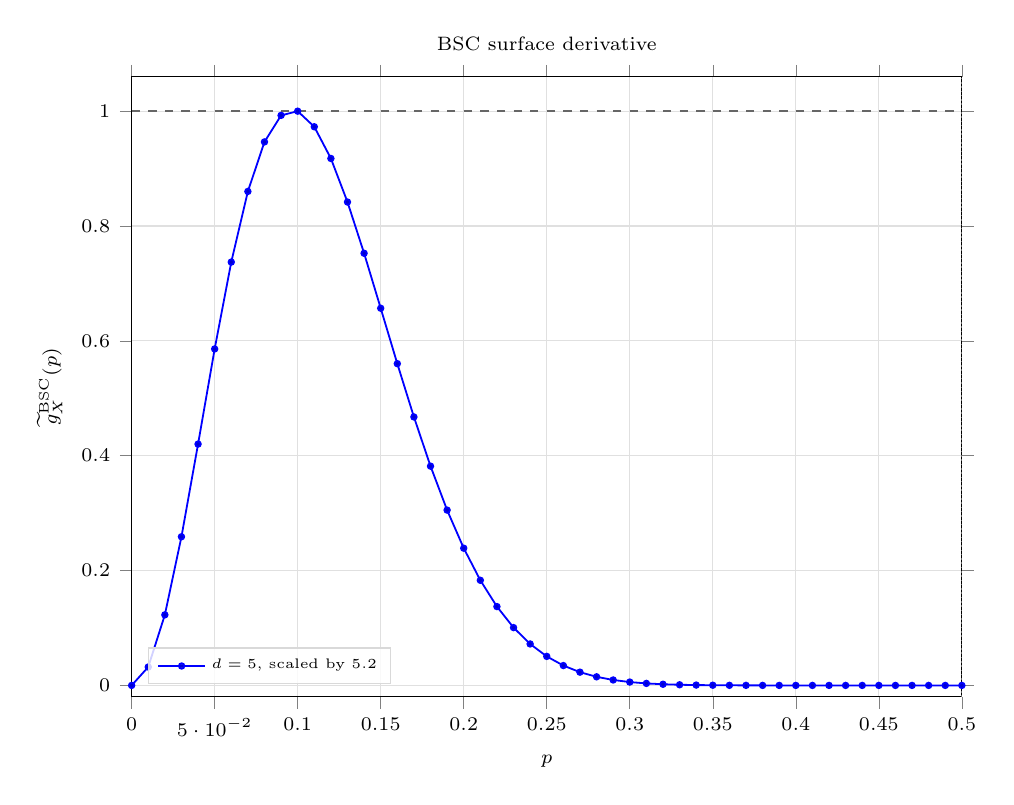
\begin{tikzpicture}
\begin{axis}[
  name=scaledBSCGEXITSurfaceFiveAxis,
  width=\linewidth,
  height=0.78\linewidth,
  title={BSC surface derivative},
  title style={font=\scriptsize},
  xlabel={$p$},
  ylabel={$\widetilde g_X^{\rm BSC}(p)$},
  xmin=0, xmax=0.5,
  ymin=-0.02, ymax=1.06,
  grid=both,
  major grid style={black!12},
  minor grid style={black!6},
  tick align=outside,
  tick label style={font=\scriptsize},
  label style={font=\scriptsize},
  legend cell align={left},
  legend style={draw=black!15, fill=white, fill opacity=0.82, text opacity=1, at={(0.02,0.02)}, anchor=south west, font=\tiny},
]
\addplot[black!60, densely dotted, line width=0.55pt, forget plot] coordinates {(0.5,-0.02) (0.5,1.06)};
\addplot[black!60, dashed, line width=0.55pt, forget plot] coordinates {(0,1) (0.5,1)};
\addplot+[color=blue, mark=*, mark size=1.0pt, line width=0.65pt]
coordinates {(0,0) (0.01,0.0320911170938) (0.02,0.122890070095) (0.03,0.258900901837) (0.04,0.420291159881) (0.05,0.585947540966) (0.06,0.737251807319) (0.07,0.860254584422) (0.08,0.946472106143) (0.09,0.992668030057) (0.1,1) (0.11,0.97286159285) (0.12,0.917671295728) (0.13,0.841776104098) (0.14,0.75256280766) (0.15,0.656811741812) (0.16,0.560287111447) (0.17,0.467533223779) (0.18,0.381833935161) (0.19,0.305289809424) (0.2,0.238970668925) (0.21,0.183107740615) (0.22,0.137297468147) (0.23,0.100696914169) (0.24,0.0721976842889) (0.25,0.0505710582817) (0.26,0.034581421041) (0.27,0.0230682633002) (0.28,0.0149992013566) (0.29,0.009497897124) (0.3,0.00585163980121) (0.31,0.00350377821497) (0.32,0.00203618765917) (0.33,0.00114651458088) (0.34,0.000624113547412) (0.35,0.000327506243873) (0.36,0.000165048921021) (0.37,7.9488723656e-05) (0.38,3.63496702417e-05) (0.39,1.56501835226e-05) (0.4,6.27310297431e-06) (0.41,2.30578472947e-06) (0.42,7.61184935473e-07) (0.43,2.19125038553e-07) (0.44,5.26677528239e-08) (0.45,9.87778526738e-09) (0.46,1.29028970427e-09) (0.47,9.48425982465e-11) (0.48,2.42976217583e-12) (0.49,4.69677276469e-15) (0.5,0)};
\addlegendentry{$d=5$, scaled by $5.2$}
\end{axis}
\end{tikzpicture}
